\documentclass[]{article}

\usepackage[top=1in, bottom=1.25in, left=0.9in, right=0.9in]{geometry}
\usepackage{titlesec}
\titleformat{\section}
  {\normalfont\Large}
  {\thesection}{1em}{}
\titleformat{\subsection}
  {\normalfont\large}
  {\thesection}{1em}{}
\usepackage{wallpaper}
\ThisURCornerWallPaper{1.0}{img/cover.png}
\usepackage{color}
\usepackage{xcolor}
\usepackage{hyperref}
\definecolor{blue}{rgb}{0.01, 0.28, 1.0}
\definecolor{lightgray}{rgb}{0.95, 0.95, 0.95}
\hypersetup{colorlinks=true, urlcolor=blue, citecolor=blue, filecolor=blue, linkcolor=blue}
\makeatletter
\renewcommand{\maketitle}{\bgroup\setlength{\parindent}{0pt}
\begin{flushleft}
	\vspace{0.5cm}
 	\huge{\@title}\vspace{0.5cm}\\
	\quad\Large Homework (Session 2)\vspace{0.5cm}\\
  	\qquad\large\textit{\@author}
\end{flushleft}\egroup
}
\makeatother
\newcommand{\fakesection}[1]{
	\section*{#1}
	\par\refstepcounter{section}
	\addcontentsline{toc}{section}{#1}
}
\newcommand{\fakesubsection}[1]{
	\subsection*{#1}
	\par\refstepcounter{subsection}
	\addcontentsline{toc}{subsection}{\protect\numberline{\thesubsection}#1}
}
\newcommand{\fakesubsubsection}[1]{
	\subsubsection*{#1}
	\par\refstepcounter{subsubsection}
	\addcontentsline{toc}{subsubsection}{#1}
}
\newcommand{\parx}{\par\noindent}
\usepackage{tikz}
\usepackage{listings}
\usepackage{amssymb}

\usepackage[cachedir=minted]{minted}

\begin{document}

\title{Category Theory for Programmers}
\author{Bruno Vandekerkhove}
\date{}
\maketitle
\vspace{0.5cm}

\tableofcontents

\fakesection{Challenges}

\fakesubsection{Chapter 3}

\fakesubsubsection{What Kind of Order?}

For a set of sets with an \textit{inclusion} relation it holds that $A\leq B, B\leq A\Rightarrow A=B$. If two sets do not share any elements, then they are not related. Which means we're dealing with a partial order.\\

\parx In \texttt{C++} you can use template functions to define functions that take a pointer to any type. A template function \texttt{min} that takes two pointers to scalar types, for example. You could pass that function a pointer to an \texttt{int} or a \texttt{long}, the compiler won't complain.

\begin{minted}[xleftmargin=20pt,linenos]{C}
#include <iostream>

template <class T, class U>
auto min(T *a, U *b) {
    return (*a < *b ? *a : *b);
}

int main(int argc, const char * argv[]) {
    int a = 1;
    long b = 2;
    printf("%i", (int)min(&a, &b));
    return 0;
}
\end{minted}

This does not work in general ; because of the strong typing system, any function that explicitly asks for a pointer to an \texttt{int} will not accept a pointer to a \texttt{long} unless you typecast. \texttt{void} is one exception. If you consider \texttt{void} a type, then any other type is one of its subtypes. Inheritance also makes it possible to substitute one type for another, presuming that the substituted class is a parent class and its substitute one of its subclasses (or subtypes). But in no case can you go the other way around ; you cannot hand a pointer to \texttt{void} to a function expecting a pointer to an \texttt{int}, for example. \\

\parx All of this implies that - if we go by \textit{naming equivalence} - then we appear to be dealing with a partial order. Naming equivalence means that two \texttt{structs} with the exact same structure are considered different types simply because of having a different name (in contrast with \textit{structural equivalence}).

\fakesubsubsection{Addition Modulo 3}

Adding 0 corresponds to the identity function, adding 1 or 2 are other possible morphisms, and any composition of these leads to the same set of morphisms (for example, composing the addition of 1 and 2 gives the identity function).

\begin{center}
\begin{tikzpicture}
	\node at (-2.5,5) (3) {$\mathbb{N}$};
	\draw[->,shorten >=1pt] (3) to [out=180,in=-90,loop,looseness=15] node[left]{$id$} (3);
	\draw[->,shorten >=1pt] (3) to [out=180,in=-90,loop,looseness=30] node[left]{$add1mod3$} (3);
	\draw[->,shorten >=1pt] (3) to [out=180,in=-90,loop,looseness=45] node[left]{$add2mod3$} (3);
\end{tikzpicture}
\end{center}

\fakesubsection{Chapter 4}

It is asked to construct and implement the Kleiski category for partial functions.

\fakesubsubsection{Construction}

The objects of the category are the types of the programming language. \\

\parx The (partial) functions take a value of a given class and return an optional. Composition of functions works as follows. The first function is called on the input. If the result is valid (i.e. a valid optional is returned) then the second function is called on the value of the returned optional. Finally, the result of this second function call is returned. If the result of the first function call wasn't valid, an invalid optional is returned. The output class of the first function has to be the same as the input class of the second one.\\

\parx The identity morphism for an optional of a given class returns the optional itself.

\fakesubsubsection{Implementation}

Below you can find an implementation in Haskell.

\newpage

\begin{minted}[xleftmargin=20pt,linenos]{haskell}
data Optional a = Valid a | Invalid deriving Show

(>=>) :: (a -> Optional b) -> (b -> Optional c) -> (a -> Optional c)
(>=>) f g = \x ->
    let y = f x
    in  case y of
        Valid z -> g z
        _ -> Invalid

return :: a -> Optional a
return x = Valid x
\end{minted}

\fakesubsubsection{Composition}

In the implementation hereafter, calling \texttt{safe\_root\_reciprocal} will result in an \texttt{Invalid} value if the input argument is either negative or equal to zero.

\begin{minted}[xleftmargin=20pt,linenos]{haskell}
safe_root :: Double -> Optional Double
safe_root x = if (x >= 0) then Valid (sqrt(x)) else Invalid

safe_reciprocal :: Double -> Optional Double
safe_reciprocal x = if (x /= 0) then Valid (1/x) else Invalid

safe_root_reciprocal = safe_reciprocal >=> safe_root
\end{minted}

\fakesubsection{Chapter 5}

\fakesubsubsection{Product \& Coproduct in Posets}

We start from any given poset with a relation denoted with `less than'. While a preorder is a `thin' category (there's at most one morphism from any object to an other one), a partial order also imposes the absence of cycles. Let's consider two objects $A$ and $B$. We want a product $C$ which has projections to $A$ and $B$ (this means it is related to them or `less than' them). Let's say there is an other object $C'$ which also has such projections.

\begin{center}
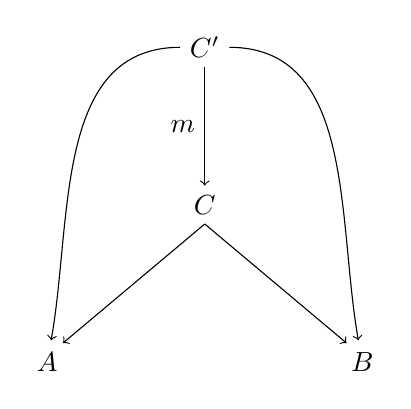
\begin{tikzpicture}
%\begin{scope}[yscale=1,xscale=-1]
	\node at (0,2) (1) {\textbf{$C$}};
	\node at (0,4) (4) {\textbf{$C'$}};
	\node at (-2,0) (2) {\textbf{$A$}};
	\node at (2,0) (3) {\textbf{$B$}};
	\draw [->] (1.south) -- ([xshift=2mm] 2.north) node[midway,right] {};
	\draw [->] (1.south) -- ([xshift=-2mm] 3.north) node[midway,left] {};
	\draw[->,shorten >=1pt] (4) to [out=0,in=100,looseness=1] node[left]{} (3);
	\draw[->,shorten >=1pt] (4) to [out=180,in=80,looseness=1] node[left]{} (2);
	\draw [->] (4.south) -- (1.north) node[midway, left] {$m$};
\end{tikzpicture}
\end{center}

Then by the definition of a product there must be a unique morphism from $C'$ to $C$ ($C'$ is `less than' $C$). This functions as a factorising function $m$. Meaning that $C$ is a `better' fit for a product than $C'$. Or in general, the product of two objects in a poset is the `largest' object that is smaller than both of these objects. Because the product in categories is unique up to isomorphism, the product in a poset must be unique. \\

\parx If we were to deal with a total order (in which any two objects including $A$ and $B$ are related), then the product of two objects would be the `smallest' of the two.

\begin{center}
\begin{tikzpicture}
%\begin{scope}[yscale=1,xscale=-1]
	\node at (-1.5,2) (1) {\textbf{$C'$}};
	\node at (-2,0) (2) {\textbf{$A$}};
	\node at (2,0) (3) {\textbf{$B$}};
	\draw [->] (1.south) -- ([xshift=1mm] 2.north) node[midway,left] {$m$};
	\draw [->] ([xshift=2mm, yshift=1mm] 1.south) -- ([xshift=-2mm] 3.north) node[midway,left] {};
	\draw [->] (2.east) -- ([xshift=-2mm] 3.west) node[midway,right] {};
	\draw[->,shorten >=1pt] (2) to [out=180,in=-90,loop,looseness=10] node[left]{$id$} (2);
\end{tikzpicture}
\end{center}

\parx The same reasoning can be applied to the coproduct, where the resulting object is the `smallest` of all objects that is `larger' than the two given objects. Or the supremum, if you will.

\fakesubsubsection{Better Coproducts (\texttt{Either} versus \texttt{int})}

It's easy to use Milewski's own factoriser function to show that you can factorise the injections to \texttt{int} :

\begin{minted}[xleftmargin=20pt,linenos]{haskell}
-- Create factorizer

i :: Int -> Int
i = id

j :: Bool -> Int
j b = if b then 1 else 0

factorizer :: (a -> c) -> (b -> c) -> Either a b -> c
factorizer i j (Left a) = i a
factorizer i j (Right b) = j b

m = factorizer i j

-- GHCI
-- m (Left 1) --> 1
-- m (Right True) --> 1
-- m (Right False) --> 0
\end{minted}

\noindent Because of the existence of such a factoriser it's clear that \texttt{Either} is a better coproduct. You cannot do the same the other way round, because 0 and 1 represent both integers and booleans (you can't factorise). I'd argue that since \texttt{int} has limited range, adding 2 to positive integers wouldn't solve this problem ; it may lead to an overflow so the injections aren't actually functions.

% 
% References
%
%\bibliographystyle{plain}
%\bibliography{References}
%\addcontentsline{toc}{section}{References}

\end{document}